\chapter{Distance Measures}
\label{ch:lesson07}

``Distance'' on a pixel grid is not as simple as it sounds. This chapter looks at three different flavors:
\begin{enumerate}
  \item \textbf{Point-to-point distance metrics} (Manhattan, chessboard, and Euclidean) --- which measure how far apart two pixels are.
  \item \textbf{Curve-length estimators} (Freeman and a refined weighted estimator) --- which measure the length of a \emph{digitized curve} (e.g.\ the boundary of a blob) from its chain code.
  \item \textbf{Chamfer distance transform} --- a fast, image-wide approximation that gives every pixel its distance to the nearest member of a given set (e.g.\ the foreground), computed with two raster-scan passes.
\end{enumerate}

\section{Point-to-point distance metrics}

Given two pixels $p=(x_1,y_1)$ and $q=(x_2,y_2)$, let $d_x=x_2-x_1$ and $d_y=y_2-y_1$. Three common metrics:
\begin{itemize}
  \item \textbf{Manhattan / city-block ($L_1$)}: distance if you can move only along the grid axes.
    \begin{equation}
    D_4(p,q) = |d_x| + |d_y|
    \end{equation}
  \item \textbf{Chessboard ($L_\infty$)}: number of king moves on a chessboard (diagonal steps are free).
    \begin{equation}
    D_8(p,q) = \max(|d_x|,\,|d_y|)
    \end{equation}
  \item \textbf{Euclidean ($L_2$)}: ordinary straight-line distance.
    \begin{equation}
    D_E(p,q) = \sqrt{d_x^2+d_y^2}
    \end{equation}
\end{itemize}
The names $D_4$ and $D_8$ come from each being the shortest path length when only 4-connected (axis) or 8-connected (axis $+$ diagonal) moves are allowed, one unit per move.

\begin{lstlisting}
def manhattan(dx, dy):  return np.abs(dx) + np.abs(dy)
def chessboard(dx, dy): return np.maximum(np.abs(dx), np.abs(dy))
def euclidean(dx, dy):  return np.sqrt(dx**2 + dy**2)
\end{lstlisting}

For every pixel in a grid, computing its distance to the center pixel under each metric and displaying it as an image (Figure~\ref{fig:l07-1}) shows the metrics agree only along the axes --- everywhere else they diverge.

\begin{figure}[h]
\centering
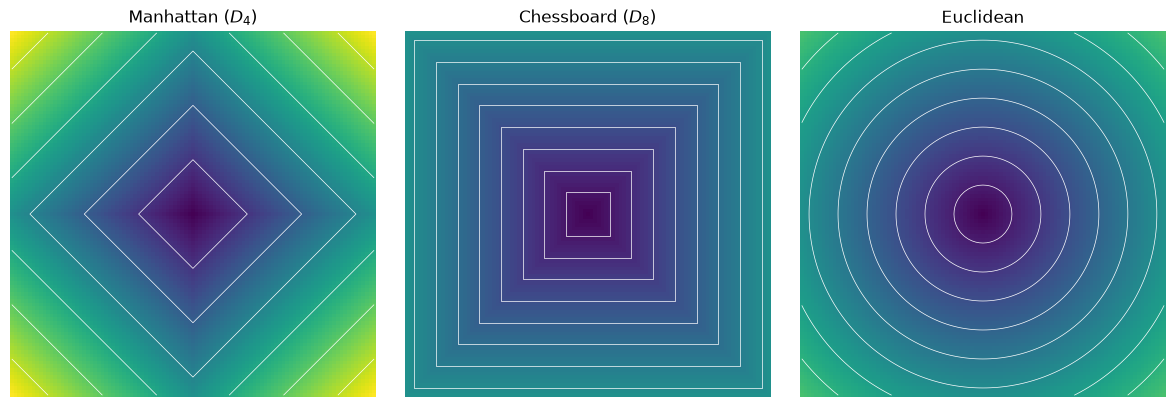
\includegraphics[width=0.95\textwidth]{figures/lesson07_fig01.png}
\caption{Distance fields for the three metrics, contoured. Manhattan distance forms diamonds, chessboard distance forms squares, and Euclidean distance forms circles --- the shape most people intuitively think of as ``equal distance away.''}
\label{fig:l07-1}
\end{figure}

\section{Estimating curve length from a chain code}

Now suppose we want to estimate the length of a \emph{curve}, not just the distance between two points. A test circle of known radius $60$ has known circumference $120\pi \approx 377$; its number of boundary pixels ($336$) is already a poor estimate, since $336 \ne 377$.

A \textbf{Freeman chain code} describes a digital curve as a sequence of unit steps in 8 possible directions ($0$--$7$, $45^\circ$ apart). Four directions are \emph{even} (horizontal/vertical, true length 1) and four are \emph{odd} (diagonal, true length $\sqrt2$). If a curve's chain code has $N_e$ even steps and $N_o$ odd steps, \textbf{Freeman's estimate} of its length is
\begin{equation}
L_{\text{Freeman}} = N_e + \sqrt{2}\,N_o.
\end{equation}
This systematically \emph{overestimates} smooth curves: a digitized circle's boundary alternates through many short zig-zag ``staircase'' steps that add up to more than the true arc length. Replacing the exact weights $(1,\sqrt2)$ with weights $(a,b)$ tuned to minimize average error over many digitized curves --- an idea sometimes associated with Kimura's chain-code length correction, with commonly cited values $a\approx0.948$, $b\approx1.343$ --- gives
\begin{equation}
L_{\text{corrected}} = a\,N_e + b\,N_o.
\end{equation}

\begin{lstlisting}
steps = np.diff(np.vstack([pts, pts[:1]]), axis=0)
is_diagonal = (steps[:, 0] != 0) & (steps[:, 1] != 0)
N_o, N_e = int(is_diagonal.sum()), int((~is_diagonal).sum())

L_freeman   = N_e + np.sqrt(2) * N_o
L_corrected = 0.948 * N_e + 1.343 * N_o
\end{lstlisting}

For radius 60 (true circumference $377.0$, $192$ even steps and $144$ odd steps): the Freeman estimate comes to $395.6$ (an error of $+4.9\%$), while the corrected estimate comes to $375.4$ (an error of just $-0.4\%$) --- much closer to the truth, without needing anything more than a count of even and odd steps.

\section{Chamfer distance transform}

Unlike the point-to-point metrics in Part 1, which measure the distance between two specific pixels, a \textbf{distance transform} labels \emph{every} pixel of a binary image with its distance to the nearest member of a given set of pixels --- typically the foreground, or the background --- useful for skeletonization, shape matching, and path planning. Computing it \emph{exactly} with Euclidean distance requires comparing every pixel against every pixel in that set (slow), or a more careful algorithm.

The \textbf{chamfer distance transform} is a fast approximation: instead of a single global search, it propagates local distances across the image in just two raster-scan passes (top-left to bottom-right, then bottom-right to top-left), adding a small fixed cost for each step to a neighbor. Using integer weights $a=3$ for axis-aligned neighbors and $b=4$ for diagonal neighbors (then dividing by 3 at the end) gives the classic \textbf{3-4 chamfer distance} --- the same idea as the Freeman/corrected chain-code weights above, but applied to every pixel instead of just a boundary. \code{cv2.distanceTransform} with \code{DIST\_L2} computes this; \code{maskSize} trades accuracy for speed.

\begin{lstlisting}
im_dist3 = cv2.distanceTransform(img, cv2.DIST_L2, maskSize=3)  # 3-4 chamfer
im_dist5 = cv2.distanceTransform(img, cv2.DIST_L2, maskSize=5)  # more accurate
\end{lstlisting}

Figure~\ref{fig:l07-2} compares the two mask sizes.

\begin{figure}[h]
\centering
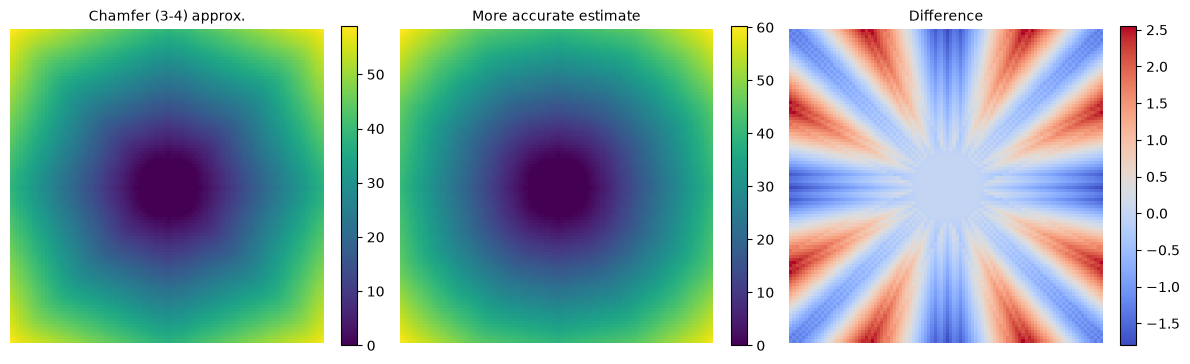
\includegraphics[width=0.95\textwidth]{figures/lesson07_fig03.png}
\caption{Chamfer (mask size 3) vs.\ a more accurate distance transform (mask size 5) and their difference; the two agree closely (max error under half a pixel).}
\label{fig:l07-2}
\end{figure}

\subsection*{Exercises}
\begin{enumerate}
  \item Repeat the circle experiment for a few different radii (e.g.\ 10, 20, 40, 80). Does the Freeman estimate's percent error stay roughly constant, or does it shrink as the circle gets bigger? Why might that be?
  \item The chessboard distance $D_8$ is the exact shortest path length when diagonal moves are allowed and cost 1. Can you construct a modified chessboard-like metric, using a diagonal cost of $\sqrt2$ instead of 1, that behaves like a coarse local version of the chain-code length estimators above? Compare it to true Euclidean distance for a few points.
\end{enumerate}

\vfill
\fullcode{lesson07}{lesson07_distance_measures}
